\section{Experimental Validation}

In an attempt to show that the model works, I created the program


\begin{figure}[H]
    \centering
    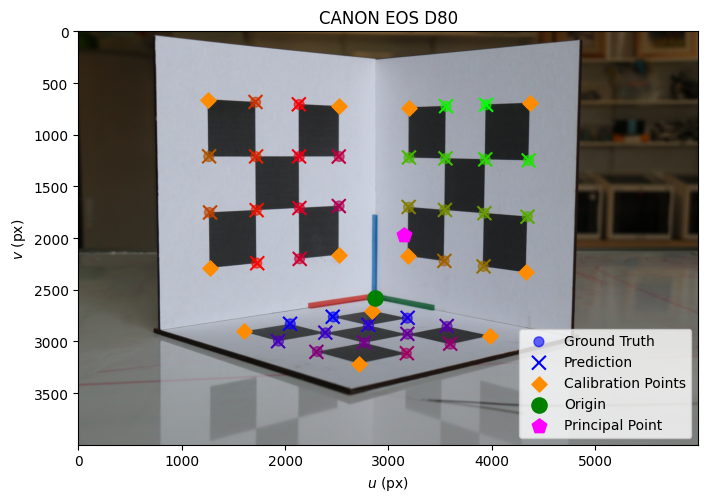
\includegraphics[width=0.8\textwidth]{assets/results/CANON EOS D80/graph.png}
\end{figure}

\begin{figure}[H]
    \centering
    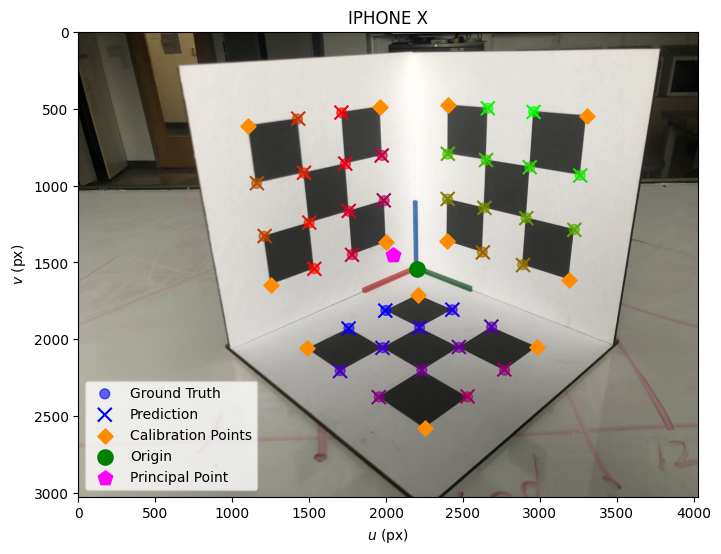
\includegraphics[width=0.8\textwidth]{assets/results/IPHONE X/graph.png}
\end{figure}

\begin{figure}[H]
    \centering
    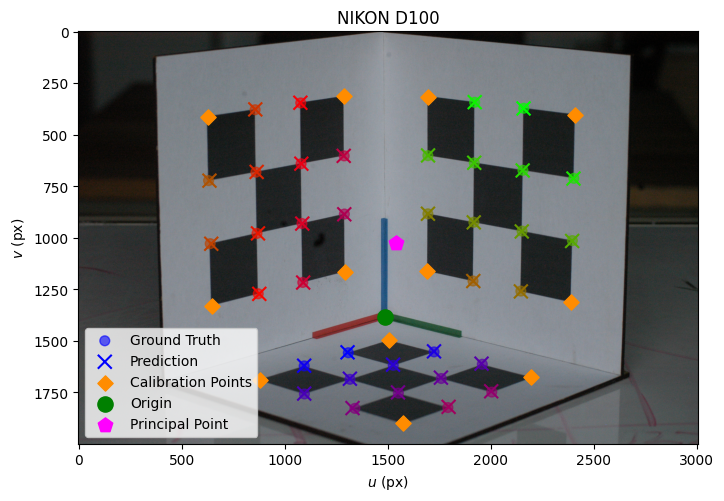
\includegraphics[width=0.8\textwidth]{assets/results/NIKON D100/graph.png}
\end{figure}

\begin{equation*}
    P =
    \begin{bmatrix}
        \num{-2.5844e-03} & \num{1.7334e-03}  & \num{-4.6719e-04} & \num{6.0581e-01} \\
        \num{4.8240e-04}  & \num{4.4097e-04}  & \num{-3.1337e-03} & \num{7.9559e-01} \\
        \num{-3.3990e-07} & \num{-3.1311e-07} & \num{-2.8179e-07} & \num{4.1340e-04}
    \end{bmatrix}
\end{equation*}

\begin{table}[H]
    \centering
    \resizebox{\columnwidth}{!}{
    \begin{tabular}{p{3cm}ccccccc}
        \toprule
                                                         &             & \multicolumn{2}{c}{\textbf{\small CANON D80}} & \multicolumn{2}{c}{\textbf{\small IPHONE X}} & \multicolumn{2}{c}{\textbf{\small NIKON D100}}                                                                               \\
        \cmidrule(lr){3-4}
        \cmidrule(lr){5-6}
        \cmidrule(lr){7-8}
                                                         &             & Spreaded Out                                  & Concentrated                                 & Spreaded Out                                   & Concentrated            & Spreaded Out            & Concentrated            \\
        \midrule
        \addlinespace
        \multirow{2}{*}{\footnotesize Focal Lengths}     & $f_x$       & $\qty{8404.1}{\pixel}$                        & $\qty{8305.9}{\pixel}$                       & $\qty{3281.5}{\pixel}$                         & $\qty{3125.7}{\pixel}$  & $\qty{8144.4}{\pixel}$  & $\qty{7716.4}{\pixel}$  \\
                                                         & $f_y$       & $\qty{8387.9}{\pixel}$                        & $\qty{8338.1}{\pixel}$                       & $\qty{3279.9}{\pixel}$                         & $\qty{3137.8}{\pixel}$  & $\qty{8142.6}{\pixel}$  & $\qty{7755.5}{\pixel}$  \\
        \addlinespace
        \multirow{2}{*}{\footnotesize Principal Point}   & $c_x$       & $\qty{3151.6}{\pixel}$                        & $\qty{3400.0}{\pixel}$                       & $\qty{2043.0}{\pixel}$                         & $\qty{2031.4}{\pixel}$  & $\qty{1541.8}{\pixel}$  & $\qty{1851.5}{\pixel}$  \\
                                                         & $c_y$       & $\qty{1972.8}{\pixel}$                        & $\qty{2075.8}{\pixel}$                       & $\qty{1453.1}{\pixel}$                         & $\qty{1467.4}{\pixel}$  & $\qty{1027.9}{\pixel}$  & $\qty{1205.4}{\pixel}$  \\
        \addlinespace
        \midrule
        \addlinespace
        \multirow{3}{*}{\footnotesize Tait-Bryan Angles} & $\alpha$    & $\qty{-81.86}{\degree}$                       & $\qty{-80.32}{\degree}$                      & $\qty{-60.21}{\degree}$                        & $\qty{-60.02}{\degree}$ & $\qty{-70.83}{\degree}$ & $\qty{-67.83}{\degree}$ \\
                                                         & $\beta$     & $\qty{44.27}{\degree}$                        & $\qty{46.00}{\degree}$                       & $\qty{38.72}{\degree}$                         & $\qty{38.28}{\degree}$  & $\qty{46.44}{\degree}$  & $\qty{48.43}{\degree}$  \\
                                                         & $\gamma$    & $\qty{4.97}{\degree}$                         & $\qty{5.98}{\degree}$                        & $\qty{21.64}{\degree}$                         & $\qty{21.81}{\degree}$  & $\qty{13.89}{\degree}$  & $\qty{16.04}{\degree}$  \\
        \addlinespace
        \multirow{3}{*}{\footnotesize Translation}       & $t_x$       & $\qty{494.8}{\mm}$                            & $\qty{492.9}{\mm}$                           & $\qty{329.0}{\mm}$                             & $\qty{317.4}{\mm}$      & $\qty{840.3}{\mm}$      & $\qty{801.1}{\mm}$      \\
                                                         & $t_y$       & $\qty{537.6}{\mm}$                            & $\qty{533.5}{\mm}$                           & $\qty{321.4}{\mm}$                             & $\qty{310.2}{\mm}$      & $\qty{766.0}{\mm}$      & $\qty{726.7}{\mm}$      \\
                                                         & $t_z$       & $\qty{128.3}{\mm}$                            & $\qty{130.5}{\mm}$                           & $\qty{208.6}{\mm}$                             & $\qty{202.1}{\mm}$      & $\qty{317.2}{\mm}$      & $\qty{306.8}{\mm}$      \\
        \addlinespace
        \midrule
        \addlinespace
        \multirow{2}{*}{\footnotesize Reproj. Errors}    & $\mu_{max}$ & $\qty{11.08}{\pixel}$                         & $\qty{17.21}{\pixel}$                        & $\qty{5.58}{\pixel}$                           & $\qty{19.48}{\pixel}$   & $\qty{11.70}{\pixel}$   & $\qty{14.13}{\pixel}$   \\
                                                         & $\mu_{avg}$ & $\qty{3.56}{\pixel}$                          & $\qty{7.36}{\pixel}$                         & $\qty{2.55}{\pixel}$                           & $\qty{4.86}{\pixel}$    & $\qty{2.81}{\pixel}$    & $\qty{5.04}{\pixel}$    \\
        \addlinespace
        \bottomrule
    \end{tabular}
}



    \caption{Intrinsic and Extrinsic Parameters calculated by \texttt{calicam}.}
\end{table}

\subsection{Validating Estimated Focal Length}
Given that specification of cameras are readily available online, we can actually evaluate the accuracy of our calculated focal lengths. Assuming that the pixels are square, we estimate the focal lengths of our cameras to be the average of the horizontal and vertical focal lengths. Then, based on the manufacturer reported size of each individual pixel (known as the \emph{pixel pitch}), we can convert our estimated focal length from pixels to millimeters.

\begin{table}[H]
    \centering
    \resizebox{\columnwidth}{!}{
    \begin{tabular}{p{4.0cm}c@{\hskip 0.5cm}c@{\hskip 0.5cm}c}
        \toprule
                                      & \textbf{\small Calculated Focal Length}\tablefootnote{Pixel pitches retrieved from \url{digicamdb.com}.} & \textbf{\small Manufacturer Reported Focal Length} & \textbf{\small \% Error} \\
        \midrule
        \textbf{\small Canon EOS D80} & $(\qty{8496}{\pixel})(\qty{3.73e-3}{\milli\meter \per \pixel}) \approx \boxed{\qty{31.7}{\milli\meter}}$        & \qty{32}{\milli\meter}                & \qty{0.94}{\percent}     \\
        \textbf{\small IPhone X}      & $(\qty{3280}{\pixel})(\qty{1.22e-3}{\milli\meter \per \pixel}) \approx \boxed{\qty{4.00}{\milli\meter}}$        & \qty{4}{\milli\meter}                 & --                       \\
        \textbf{\small Nikon D100}    & $(\qty{8143}{\pixel})(\qty{7.82e-3}{\milli\meter \per \pixel}) \approx \boxed{\qty{63.7}{\milli\meter}}$        & \qty{55}{\milli\meter}                & \qty{15.6}{\percent}     \\
        \bottomrule
    \end{tabular}
}

    \caption{Comparison of Calculated vs. Reported Focal Length.}
\end{table}

Considering that the focal lengths reported by manufacturers are often only accurate to around $\pm \qty{1}{\milli\meter}$,\footcite{waynefAnswerAre2017} my results are very promising, with exception to the Nikon D100. However, this error is in fact a result of human error, as I forgot to turn off autofocus on the Nikon D100, and the zoom lens Nikon D100 altered the effective focal length. 


